\chapter{Artefakt-Design und Entwicklung}

Die Entwicklung des Artefakts folgte einem strukturierten Prozess, der sicherstellt, dass jede technische Entscheidung sowohl praxisnah als auch wissenschaftlich fundiert ist. In diesem Kapitel werden die Schritte zur Datenvorbereitung, Implementierung der Trainingspipeline und Hyperparameter-Optimierung detailliert diskutiert und begründet.

\section{Datensammlung und Analyse}

  Die vorliegende Arbeit nutzt Telemetriedaten aus der Porsche Motorsport Cloud Plattform (ADX). Es wurden sämtliche Rennsessions der IMSA- und WEC-Meisterschaften der Jahre 2023 bis 2025 extrahiert. Zur Minimierung von Varianz durch unterschiedliche Fahrsituationen beschränkt sich die Auswahl auf Rennsessions, während Trainings- und Qualifikationssessions ausgeschlossen wurden. Zusätzlich erfolgte eine Filterung auf Runden mit Trockenreifen, da Regenbedingungen weitere Einflussfaktoren einführen. Die Datenselektion wurde direkt beim Abruf mittels der ADX-Kusto Query Language (KQL) vorgenommen, wodurch ein Rohdatensatz im CSV-Format mit 17 735 Runden (Datenpunkten) resultierte.

  Im Rahmen eines Experteninterviews mit dem Performance Engineer wurden jene Parameter identifiziert, die als Merkmale (Features) in das Machine-Learning-Modell eingehen.\footnote{Vgl. Experteninterview 2 (12.09.2025)} Die Merkmale gliedern sich in kontinuierliche und kategoriale Features. Zu den kontinuierlichen Merkmalen zählen Umgebungstemperatur, Reifentemperatur je Rad, Reifendruck je Rad, Fuel Load und Tyre Mileage Laps je Rad. Kategoriale Merkmale umfassen Mechanical Balance (Anti-Roll-Bar-Front/Rear), Brake Balance, Traction Control, Tyre Compound und Track. 
  Als Zielvariable dient der durchschnittliche Untersteer-Wert pro Runde (aUndersteer\_AVG) \textbf{Berechnung in DP ergänzen}, wobei Werte über Null Untersteer und Werte unter Null Übersteer anzeigen. Alle Parameter und die Zielvariable wurden rundenmittelnd aggregiert, sodass jeder Datensatzpunkt einer einzelnen Rennrunde entspricht.

Die explorative Datenanalyse (EDA) wurde durchgeführt, um die Dateneigenschaften zu untersuchen und potenzielle Datenqualitätsprobleme zu identifizieren. Zunächst wurde die Verteilung der Zielvariable aUndersteer\_AVG untersucht. 
\begin{figure}[H]
  \centering
  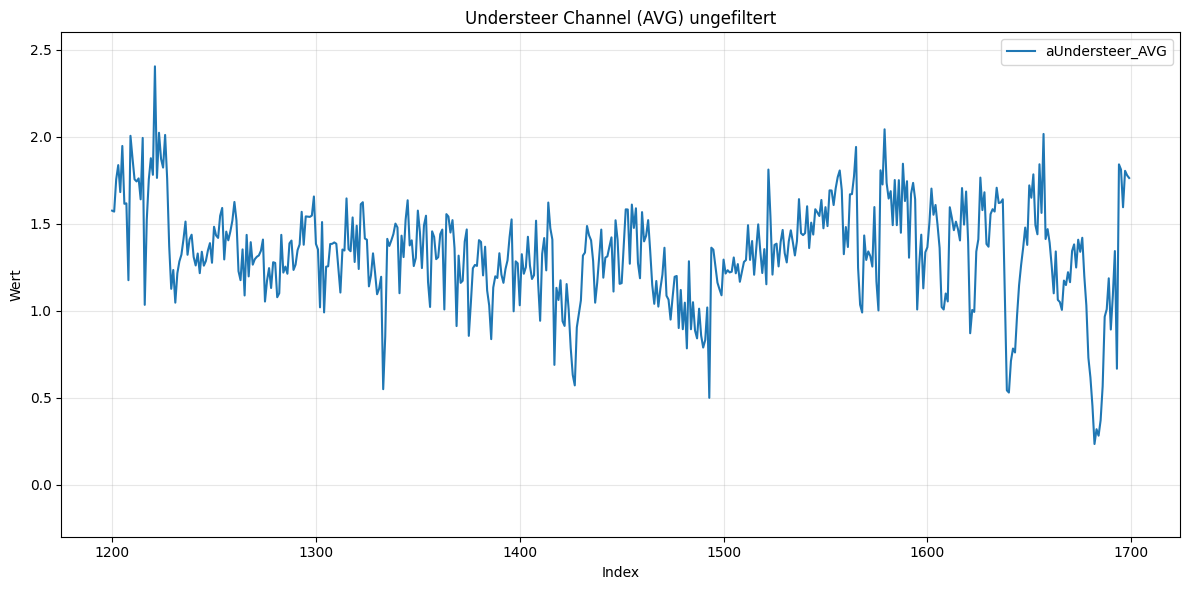
\includegraphics[width=0.8\textwidth]{graphics/understeer_nonfilt.png}
  \caption{Ausschnitt der Werte der Zielvariable aUndersteer\_AVG.}
  \label{fig:understeer_distribution}
\end{figure}
Der in Abbildung \ref{fig:understeer_distribution} dargestellte Verlauf des Understeer-Channels ist auffällig, denn obwohl es sich bereits um Durchschnitte über jeweils eine Runde handelt, weist der Graph eine hohe Volatilität auf.
Diese Erkenntnis sollte in der Modellierung der Vorverarbeitungsschritte berücksichtigt werden, um die Robustheit des Modells zu erhöhen.

Die Verteilungen der zentralen kontinuierlichen Features wurden ebenfalls untersucht. Abbildung \ref{fig:temp_distribution} zeigt exemplarisch die Verteilung der Reifentemperatur hinten-rechts. Dabei sind sowohl realistische, aber extreme Werte unter 40 Grad Celsius als auch auffällige, unrealistische Ausreißer über 300 Grad Celsius zu erkennen.\footnote{Vgl. Experteninterview 1 (29.08.2025)} Diese Ausreißer deuten auf potenzielle Sensorfehler oder Datenqualitätsprobleme hin und werden in der Datenvorbereitung entsprechend gefiltert.
\begin{figure}[H]
  \centering
  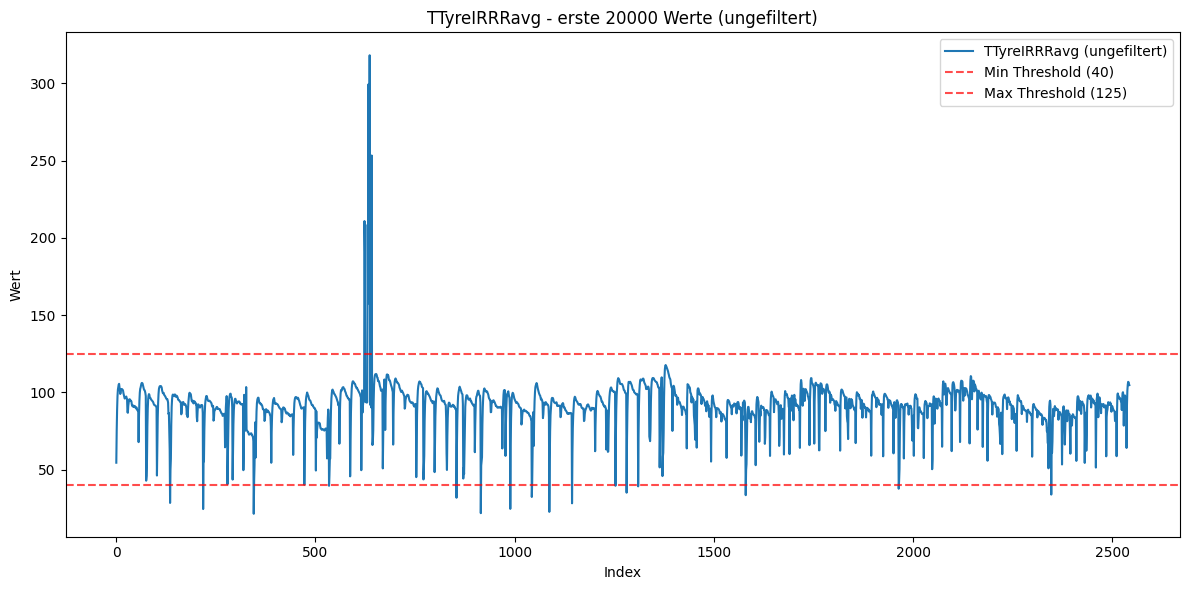
\includegraphics[width=0.8\textwidth]{graphics/TempPlot.png}
  \caption{Plot der Reifentemperatur hinten-rechts.}
  \label{fig:temp_distribution}
\end{figure}

Auch bei den Werten des Reifendrucks scheint es auffällige Ausreißer zu geben. Abbildung \ref{fig:druck_distribution} zeigt die Verteilung des Reifendrucks vorne-links. Hier sind ebenfalls unrealistische Werte zu erkennen, die auf mögliche Datenqualitätsprobleme hinweisen und in der Vorverarbeitung entsprechend berücksichtigt werden müssen.
\begin{figure}[H]
  \centering
  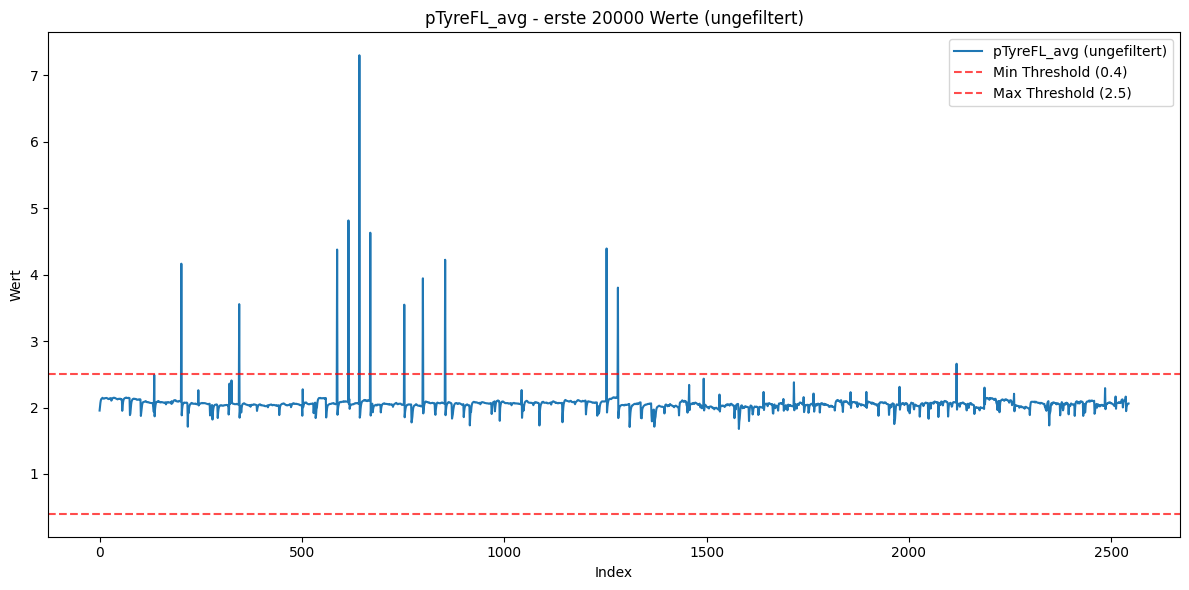
\includegraphics[width=0.8\textwidth]{graphics/DruckPlot.png}
  \caption{Plot des Reifendrucks vorne-links.}
  \label{fig:druck_distribution}
\end{figure}

Abschließend wurde mittels Korrelationsmatrix die Stärke der Zusammenhänge aller Merkmale untersucht. Dabei ergaben sich insbesondere enge Korrelationen zwischen den Reifentemperatur- und Reifendrucksensoren sowie zwischen der Kraftstoffmenge und der Anzahl der Runden pro Reifenlaufleistung. 
\begin{figure}[H]
  \centering
  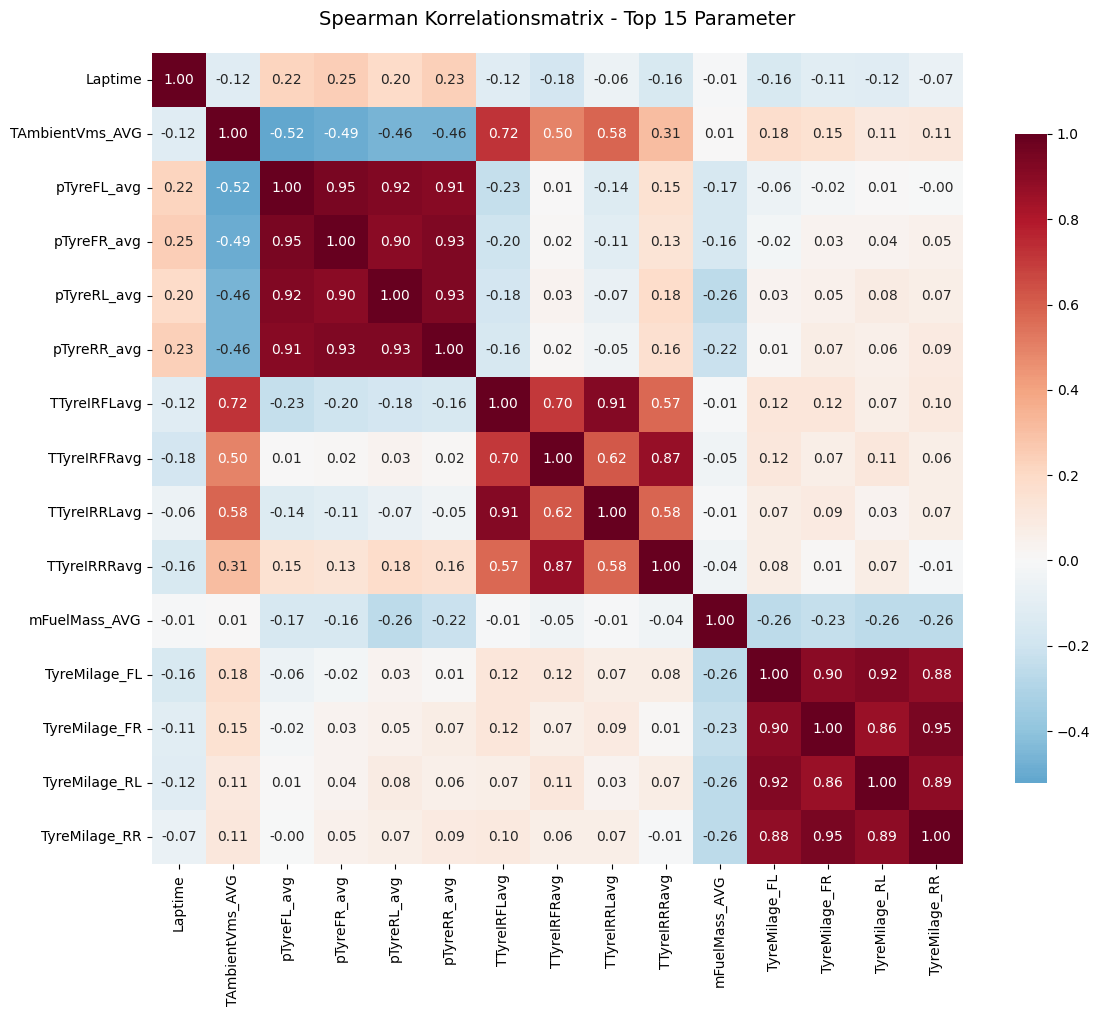
\includegraphics[width=0.8\textwidth]{graphics/korrelations_matrix_top.png}
  \caption{Korrelationsmatrix der 15 wichtigsten Parameter.}
  \label{fig:korrelations_matrix}
\end{figure}


Die explorative Analyse zeigte (i) stark schwankende Zielgrößen trotz Rundenglättung, (ii) evidente Ausreißer und Sensorartefakte bei Temperatur und Druck, sowie (iii) hohe Redundanzen in korrelierten Messkanälen (Reifen- und Drucksensorik, Fuel Load vs. Tyre Mileage). Im nächsten Abschnitt werden die daraus abgeleiteten Vorverarbeitungsschritte und das Feature-Engineering formalisiert und implementierungsorientiert beschrieben.



\section{Datenvorbereitung und Feature-Engineering}

- Aus den Erkenntnisses der EDA werden verschiedene Vorverarbeitungsschritte abgeleitet
- Ziel der Vorverarbeitung ist die Bereinigung und Optimierung des Datensatzes für das Modelltraining
- Filter kommen zum Einsatz um Sensorfehler und Extremereignisse zu entfernen
- Vorverarbeitungsschritte:
- Entfernung von Runden bei denen die Rundenzeit +- 40 Sekunden (ca. eine Standardabweichung) vom Mittelwert abweicht, weitere Reduzierung der Varianz
- Entfernung von redundanten Features (Reifentemperaturen, Reifendruck) anhand der Korrelationsmatrix und Erstellung von neuen abgeleiteten Features
- Festlegung von Thresholds für Ausreißer für Features
- Durch sehr unregelmäßigen Zielvariablen graph beschluss verschiedene Glättungen mittels gleitender Durchschnitte (Fenstergrößen 2, 3, 5, 8) und ohne zu testen
- Begründung der Glättungsentscheidungen: Die Wahl der Fenstergrößen basiert auf der Analyse der Zeitreihenstruktur der Zielvariablen. Kleinere Fenster erfassen kurzfristige Schwankungen, während größere Fenster langfristige Trends glätten.
- Umsetzung: Diese Vorverarbeitungsschritte werden in einem Skript \texttt{preprocess\_all\_events.py} implementiert.
- Der Track (Alphabestisch) zu TrackCode (numerische Codierung) und eine Mapping-Datei wird erstellt.
- One-Hot-Encoding nicht notwendig, da Baum-basierte Modelle wie XGBoost und LightGBM kategoriale Features nativ unterstützen\footnote{Vgl. Chen, Tianqi; Guestrin, Carlos 2016. XGBoost: A Scalable Tree Boosting System, in Proceedings of the 22nd ACM SIGKDD International Conference on Knowledge Discovery and Data Mining, New York ACM, S. 785-794}\footnote{Vgl. Ke, Guolin et al. 2017. LightGBM: A Highly Efficient Gradient Boosting Decision Tree, in Advances in Neural Information Processing Systems 30, La Jolla Curran Associates, S. 3146-3154}.
- Für die in Kapitel \ref{sec:validierung_modellvergleich} behandelte Validierung der Modelle werden separate Validierungsdatensätze erstellt:
- Dafür wird ein gesamtes Event nach der Leave-One-Out-Methode separiert
- Danach werden aus dem verbleibenden Datensatz 10\% zufällig ausgewählt und als Validierungsdatensatz verwendet.
- Beide Validierungsdatensätze hat das Model dem Training nicht gesehen.
- Resultierende Datensätze nach Vorverarbeitung und Aufteilung: 
- Daraus ergeben sich 10 Trainingsdatensätze: Mit und ohne kategoriale Features, jeweils mit 5 verschiedenen Glättungen (keine, 2, 3, 5, 8)
- Und 4 Validierungsdatensätze: Mit und ohne kategoriale Features, jeweils einmal für das Event und für den Zufallsdatensatz
- Resultierenden Datensatzgrößen:
- Trainingsdatensätze jeweils: ca. 9000 Runden (Datenpunkte)
- Validierungsdatensätze: Event: ca. 75 Runden (Datenpunkte) \& Zufallsdatensatz: ca. 1000 Runden (Datenpunkte)

\section{Modelltraining und Hyperparameter-Optimierung}

- Modelle: LightGBM (LGBMRegressor) und XGBoost (XGBRegressor)
- Begründung: Beide Algorithmen sind leistungsstarke, effiziente und weit verbreitete Implementierungen von Gradient Boosting Decision Trees, die sich besonders gut für strukturierte Daten eignen\footnote{Vgl. Chen, Tianqi; Guestrin, Carlos 2016. XGBoost: A Scalable Tree Boosting System, in Proceedings of the 22nd ACM SIGKDD International Conference on Knowledge Discovery and Data Mining, New York ACM, S. 785-794}\footnote{Vgl. Ke, Guolin et al. 2017. LightGBM: A Highly Efficient Gradient Boosting Decision Tree, in Advances in Neural Information Processing Systems 30, La Jolla Curran Associates, S. 3146-3154}.
- Beide Algorithmen unterstützen nativ die Verarbeitung von Kategorischen Features, was die Notwendigkeit für aufwändiges One-Hot-Encoding eliminiert und die Modellkomplexität reduziert
- Implementierung der Trainingspipeline in einem Skript \texttt{train\_model.py}
- 


Für XGBoost und LightGBM kommt ein strukturiertes GridSearchCV zum Einsatz\footnote{Vgl. Chen, Tianqi; Guestrin, Carlos 2016. XGBoost: A Scalable Tree Boosting System, in Proceedings of the 22nd ACM SIGKDD International Conference on Knowledge Discovery and Data Mining, New York ACM, S. 785-794}\footnote{Vgl. Ke, Guolin et al. 2017. LightGBM: A Highly Efficient Gradient Boosting Decision Tree, in Advances in Neural Information Processing Systems 30, La Jolla Curran Associates, S. 3146-3154}. Die Parameterbereiche sind in drei Komplexitätsstufen unterteilt:

\begin{itemize}
  \item \textbf{Shallow:} 50–100 Bäume, \texttt{max\_depth} 3–4
  \item \textbf{Medium:} 100–500 Bäume, \texttt{max\_depth} 5–9
  \item \textbf{Deep:} 300–700 Bäume, \texttt{max\_depth} 10–12
\end{itemize}

Diese Aufteilung basiert auf Benchmark-Ergebnissen, die einen Kompromiss zwischen Rechenaufwand und Modellgenauigkeit zeigen. In Gradient-Boosting-Verfahren sollten Bäume typischerweise eine geringe Tiefe zwischen 3 und 8 Ebenen haben, da vollständig gewachsene Bäume zu Overfitting führen würden\footnote{Vgl. Friedman, Jerome H. 2001. Greedy Function Approximation: A Gradient Boosting Machine, in The Annals of Statistics 29, 5, S. 1189-1232}. Schwache Lerner bei jedem Schritt helfen, Overfitting zu reduzieren\footnote{Vgl. ebd., S. 1203-1208}.

Jede Parameterkombination wird mittels dreifacher Cross-Validation über den R²-Score bewertet\footnote{Vgl. Pedregosa, Fabian et al. 2011. Scikit-learn: Machine Learning in Python, in Journal of Machine Learning Research 12, 1, S. 2825-2830}. K-Fold Cross-Validation ist die am häufigsten verwendete Methode zur Bestimmung der Wahrscheinlichkeit, dass ein Machine Learning-Ergebnis zufällig generiert wird\footnote{Vgl. Stone, Mervyn 1974. Cross-Validatory Choice and Assessment of Statistical Predictions, in Journal of the Royal Statistical Society 36, 2, S. 111-147}. Die erzielten Ergebnisse fließen in eine Tabelle mit den jeweils besten Parametern ein.

\section{Validierung und Modellvergleich}
\label{sec:validierung_modellvergleich}

Die abschließende Validierung erfolgt in einem dedizierten Jupyter-Notebook, das die finalen Modelle auf einem zuvor ungesehenen Validierungsdatensatz evaluiert und vergleichbar macht. Der Workflow gliedert sich in folgende Schritte:

\begin{itemize}
  \item \textbf{Verzeichnisstruktur und Dateipfade}\\
  Modelle liegen in Unterordnern von \texttt{../outputs/models/2/}. Zwei Validierungs-CSVs sind vorhanden: \texttt{val\_alldata.csv} (alle Features) und \texttt{val\_continuous.csv} (nur kontinuierliche Features).
  
  \item \textbf{Laden der Validierungsdaten}\\
  Für jede Modellvariante („alldata" vs. „continuous") wird das entsprechende CSV geladen. Vor der Vorhersage werden alle Spalten mit nur einem eindeutigen Wert entfernt, um irrelevante Features auszuschließen.
  
  \item \textbf{Modell-Loading und Vorhersage}\\
  In jedem Modellordner wird je ein XGBoost- (Dateiname \texttt{best\_xgb\_model.pkl}) und ein LightGBM-Modell (\texttt{best\_lgb\_model.pkl}) geladen. Mit dem jeweiligen Validierungs-Set werden Zielwerte \(y\) und Prädiktionen \(\hat{y}\) erzeugt.
  
  \item \textbf{Berechnung der Metriken}\\
  \begin{itemize}
    \item Mean Absolute Error (MAE)
    \item R²-Score (Bestimmtheitsmaß)
  \end{itemize}
  Die Ergebnisse werden in einer Tabelle \texttt{results\_df} gespeichert mit den Spalten \texttt{Modellordner}, \texttt{Modelltyp}, \texttt{Validation-CSV}, \texttt{MAE}, \texttt{R2}. Der R²-Score misst den Anteil der Varianz in der abhängigen Variable, der durch die unabhängigen Variablen vorhersagbar ist, wobei der bestmögliche Wert 1.0 beträgt\footnote{Vgl. James, Gareth et al. 2021. An Introduction to Statistical Learning. with Applications in R. 2. Aufl. New York Springer, S. 68-74}.
  
  \item \textbf{Top-5-Auswahl nach R² und MAE}\\
  \texttt{top\_r2}: die fünf besten Modelle nach absteigendem R²\\
  \texttt{top\_mae}: die fünf besten Modelle nach aufsteigendem MAE
  
  \item \textbf{Konsolidierte Rangfolge}\\
  Jedes Modell erhält einen Rang in beiden Top-5-Listen (Platz 0–4; außerhalb = 5). Aus dem Mittelwert dieser beiden Ränge wird eine finale Liste der fünf besten Modelle (\texttt{rankings\_df}) erstellt.
\end{itemize}

\noindent
Dadurch wird transparent, welche Modelltyp-/Feature-Kombination auf neuen, ungesehenen Telemetriedaten am besten generalisiert. Die Generalisierungsfähigkeit ist die Fähigkeit eines trainierten Modells, genaue Vorhersagen für neue, ungesehene Daten zu treffen\footnote{Vgl. Vapnik, Vladimir N. 2013. The Nature of Statistical Learning Theory. 2. Aufl. New York Springer, S. 15-28}.
